\documentclass[11pt]{article}
\usepackage[T1]{fontenc}
\usepackage[utf8]{inputenc}
\usepackage{amsmath,amssymb,amsthm,mathtools}
\usepackage[margin=1in]{geometry}
\usepackage{tikz}
\usetikzlibrary{arrows.meta,calc,positioning,patterns}
\usepackage{hyperref,xurl}
\newtheorem{theorem}{Theorem}[section]
\newtheorem{lemma}[theorem]{Lemma}
\newtheorem{proposition}[theorem]{Proposition}
\newtheorem{corollary}[theorem]{Corollary}
\theoremstyle{remark}
\newtheorem{remark}[theorem]{Remark}
\newcommand{\HH}{\mathbb H}
\newcommand{\VV}{\operatorname{V}}
\newcommand{\FF}{\operatorname{F}}
\newcommand{\ip}[2]{\langle #1,#2\rangle}
\title{Necessary size constraints for entirely ideal\linebreak
right-angled polytopes in dimensions five and six}
\author{Coxeter Polytopes Frontier Project}
\date{19 October 2026}
\begin{document}
\maketitle
\begin{abstract}
An entirely ideal finite-volume right-angled hyperbolic five-polytope
has at least $63$ facets and $211$ vertices. In dimension six the
corresponding bounds are $275$ facets and $6{,}106$ vertices, with
$\VV(P)\ge\lceil6039\FF(P)/272\rceil$.
The proof combines an actual outside-cusp neighbor capacity, fixed-scale
polygon identities, an exclusion of an eleven-vertex equality carrier,
and good-edge cusp transport with a sharp reciprocal estimate.
One previously proved internal small-facet theorem is stated separately
with its published three-dimensional classification input.
With the published Nikulin--Khovanskii and Dufour inequalities, the
entirely ideal five- and six-face fractions in ambient dimensions eleven
and twelve are respectively less than $4/47$ and $15/248$.
These are necessary size and incidence constraints. They neither exclude
dimensions five or six nor supply examples or a full formal proof.
\end{abstract}

\section{Scope, inputs and actual faces}\label{sec:foundations}

All polytopes are full-dimensional, convex and finite-volume. An
\emph{entirely ideal} polytope has only ideal vertices. Write $\VV(X)$
and $\FF(X)$ for its vertex and facet counts. Faces of dimension at least
three inherit finite volume and right angles; two-faces are ideal polygons.
At an ideal vertex of an
$n$-dimensional right-angled polytope the horospherical link is a
rectangular $(n-1)$-box; its $2^{n-1}$ vertices give the graph degree.
The polytope is simple at the relative interior of every positive-
dimensional face. These standard geometric facts, and acuteness of all
actual outward wall normals, are our foundational inputs.

We use the Lorentz model with future timelike vectors of negative square
and outward unit spacelike normals $n_i$. Thus
$P=\{x\in\HH^n:\ip{x}{n_i}\le0\}$ and distinct actual normals have
nonpositive products, including facets not sharing a visible ridge.
The following all-wall argument will be used throughout.

\begin{lemma}[Acute projection and the wall-product gap]\label{lem:projection}
Suppose selected actual normals have positive-definite Gram matrix $M$
with entrywise nonnegative inverse. Their common hyperplanes meet $P$
in an actual face, with all other walls strict at a finite relative-
interior point. In a right-angled polytope, distinct actual unit normals
therefore have product either zero or at most $-1$.
In an entirely ideal $n$-polytope, $n$ mutually orthogonal actual normals
cannot occur.
\end{lemma}
\begin{proof}
Choose a strict future timelike interior point $q$. With
$b_i=\ip{q}{n_i}<0$ and $a=M^{-1}b$, put $p=q-\sum_i a_i n_i$.
Every $a_i<0$, the selected products vanish, and
\[
 p^2=q^2-b^TM^{-1}b<0,\qquad
 \ip{p}{n_j}=\ip{q}{n_j}-\sum_i a_i\ip{n_i}{n_j}<0
\]
for any other actual wall. Also $\ip{q}{p}<0$, so $p$ is future.
After normalization it is the asserted actual point. In particular a
two-root product in $(-1,0)$ would give an actual nonright ridge, and
$n$ orthogonal roots would give an actual finite vertex.
\end{proof}

A positive null combination of actual outward normals is nonzero
because its product with $q$ is negative. Its ray is future and feasible
against every other wall by acuteness. Compact sections or assertions
about feasible edges below will always include this all-wall condition.

\begin{lemma}[Facet injection]\label{lem:injection}
For an entirely ideal facet $A$ of an entirely ideal right-angled $P$,
\begin{equation}\label{eq:facetInjection}
 \FF(P)\ge1+\FF(A)+\VV(A).
\end{equation}
\end{lemma}
\begin{proof}
Count $A$, its distinct ridge-neighbor facets, and at each vertex $u$
of $A$ the unique actual facet opposite $A$ in the rectangular cusp
link. A cusp-opposite hyperplane is asymptotic to $A$ at $u$ only, so
it cannot serve two different cusps. Nor can it be a ridge neighbor,
whose hyperplane is orthogonal to $A$.
\end{proof}

For an ideal right-angled three-polyhedron with $m$ vertices, degree four
and Euler give $2m$ edges and $m+2$ polygonal faces. If $p_k$ counts
its $k$-gonal faces, then
\begin{equation}\label{eq:threeEuler}
 p_3-\sum_{k\ge5}(k-4)p_k=8.
\end{equation}
In particular it has at least six vertices and eight triangular faces.
These elementary identities need no classification.

\section{The outside-cusp capacity}\label{sec:capacity}

\begin{lemma}\label{lem:capacity}
An ideal vertex outside a facet $A$ of an entirely ideal right-angled
$n$-polytope has at most two graph-neighbors in $A$. Consequently
\begin{equation}\label{eq:capacityprop}
 \VV(P)\ge\bigl(1+2^{n-3}\bigr)\VV(A).
\end{equation}
\end{lemma}
\begin{proof}
Send the outside vertex $w$ to infinity. Its incident vertical walls
bound $\prod_{i=1}^{n-1}[0,L_i]$. The wall of $A$ is a hemisphere of
center $c$ and radius $R$, with $P$ outside its ball. Its unit-normal
products with the two coordinate walls are $-c_i/R$ and
$(c_i-L_i)/R$. Lemma~\ref{lem:projection} implies
\begin{equation}\label{eq:coordinategap}
 c_i\in\{0\}\cup[R,\infty),\qquad
 L_i-c_i\in\{0\}\cup[R,\infty).
\end{equation}
An edge from $w$ is vertical over a box corner $\xi$. If its other
endpoint lies on $A$, then $\sum_i(\xi_i-c_i)^2=R^2$.
Every nonzero summand's absolute coordinate difference is at least $R$
by \eqref{eq:coordinategap}. Exactly one is nonzero, and equals $R$.
Thus $c$ lies on all but at most one boundary coordinate hyperplane.
It cannot be a box corner: $A$ and those $n-1$ vertical walls would
be mutually orthogonal actual walls, forcing an actual finite vertex.
Therefore $c$ is in the relative interior of one box edge; only its
two endpoints can satisfy the sphere equation. If there is no neighbor,
no assertion about the position of $c$ is needed.

At a vertex of $A$, precisely $2^{n-2}$ edges leave $A$, by comparing
its two box links. Their other endpoints lie outside $A$: an edge
whose endpoints lie in a face lies in that face. Counting outgoing
edges against the proved capacity gives
$2^{n-2}\VV(A)\le2(\VV(P)-\VV(A))$.
\end{proof}

\begin{figure}[tb]
\centering
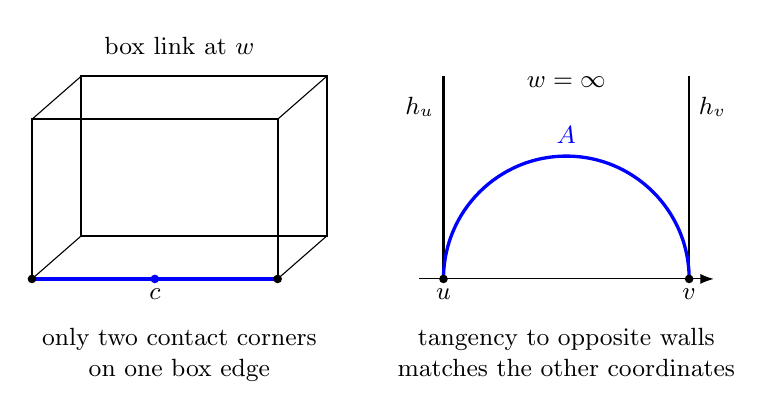
\begin{tikzpicture}[scale=.78,>=Latex,font=\small]
 \begin{scope}[xshift=-4.2cm]
  \draw[thick] (0,0) rectangle (4,2.6);
  \draw[thick] (.8,.7) rectangle (4.8,3.3);
  \draw (0,0)--(.8,.7) (4,0)--(4.8,.7)
        (4,2.6)--(4.8,3.3) (0,2.6)--(.8,3.3);
  \draw[very thick,blue] (0,0)--(4,0);
  \fill[blue] (2,0) circle(2pt);
  \fill (0,0) circle(2pt) (4,0) circle(2pt);
  \node[below] at (2,0) {$c$};
  \node[above] at (2.4,3.5) {box link at $w$};
  \node[below,align=center] at (2.4,-.65)
       {only two contact corners\\on one box edge};
 \end{scope}
 \begin{scope}[xshift=2.5cm]
  \draw[->] (-.4,0)--(4.4,0);
  \draw[thick] (0,0)--(0,3.3) (4,0)--(4,3.3);
  \draw[blue,very thick] (4,0) arc[start angle=0,end angle=180,radius=2];
  \fill (0,0) circle(2pt) (4,0) circle(2pt);
  \node[below] at (0,0) {$u$}; \node[below] at (4,0) {$v$};
  \node[left] at (0,2.8) {$h_u$};
  \node[right] at (4,2.8) {$h_v$};
  \node[blue] at (2,2.35) {$A$};
  \node at (2,3.2) {$w=\infty$};
  \node[below,align=center] at (2,-.65)
       {tangency to opposite walls\\matches the other coordinates};
 \end{scope}
\end{tikzpicture}
\caption{The capacity argument (left, a box-link schematic) and the
two-dimensional section used in the actual tangency argument (right).
The latter is applied only after both tangency points are actual vertices.}
\label{fig:box}
\end{figure}

\section{Fixed-scale polygon identities}\label{sec:polygon}

Let $A$ be a facet of an ideal right-angled polytope, with unit normal
$n$. At each vertex $u$ let $h_u$ be its actual cusp-opposite facet and
put $t_u=n+h_u$. This is a future null vector perpendicular to $n$,
with scale fixed by the two unit normals. Distinct $u$ give distinct
$h_u$. For an edge $uv$ of $A$, its other supporting normals are
orthogonal to both $h_u,h_v$. If these were orthogonal as well,
Lemma~\ref{lem:projection} would give a finite ambient vertex. Hence
\begin{equation}\label{eq:edgeproduct}
 -\ip{t_u}{t_v}=1-\ip{h_u}{h_v}\ge2.
\end{equation}

At a cusp of $A$, each opposite pair of intrinsic unit facet normals
has positive sum $\alpha t_u$. A corner of a polygonal two-face uses
one such pair; its intrinsic normals remain unit because they are
orthogonal to the supporting walls. The following statements use this
same scale at every corner, not freely rescaled null representatives.

\begin{lemma}[Small corners]\label{lem:polygon}
Every polygonal two-face of $A$ has at least two corner coefficients
$\gamma<2$. If a triangular face has consecutive null products $-2$,
all three coefficients are one.
\end{lemma}
\begin{proof}
In the polygon's Lorentz plane use
\[
 T(a,b)=(a^2+b^2,a^2-b^2,2ab),\qquad
 \ip{T(v)}{T(w)}=-2\det(v,w)^2.
\]
Choose cyclic projective lifts $v_i$ with $t_i=T(v_i)$ and signs
$v_0=-v_k$, $v_{k+1}=-v_1$. The successive determinants
$\ell_i=\det(v_i,v_{i+1})$, including the lifted last gap, are positive
and at least one by \eqref{eq:edgeproduct}. A direct side-normal
calculation gives
\begin{equation}\label{eq:spinor}
 \gamma_i=\frac{\det(v_{i-1},v_{i+1})}{\ell_{i-1}\ell_i},\qquad
 \frac{v_{i-1}}{\ell_{i-1}}+
 \frac{v_{i+1}}{\ell_i}=\gamma_i v_i.
\end{equation}
For example send $v_i$ to $(1,0)$ and write its neighbors as
$(a,-\ell_{i-1})$, $(b,\ell_i)$. The outward side normals are
$(a/\ell_{i-1},a/\ell_{i-1},-1)$ and $(b/\ell_i,b/\ell_i,1)$;
their sum is exactly $\gamma_i T(1,0)$.

The symmetric recurrence matrix has diagonal $\gamma_i$, off-diagonal
$-1/\ell_i$, and positive wrap entries $1/\ell_k$. Its kernel contains
the two independent spinor coordinate arrays. If at most one diagonal
were below two, delete that index, or any index if none is below two.
The remaining path matrix is positive definite: its quadratic form
dominates
\[
 x_1^2+x_{k-1}^2+
 \sum_{j=1}^{k-2}(|x_j|-|x_{j+1}|)^2>0
\]
for nonzero $x$. Its rank $k-1$ contradicts the two kernel vectors.
This includes $k=3$, with the indicated wrap sign. For a triangle with
all $\ell_i=1$, formula~\eqref{eq:spinor}, or the three pair-sum
products, gives $\gamma_i\gamma_j=1$ and hence all $\gamma_i=1$.
\end{proof}

\begin{lemma}[A decorated quadrilateral]\label{lem:quad}
If all four consecutive null products on a quadrilateral equal $-2$,
its corner coefficients alternate $B,2/B,B,2/B$. For the two opposite
corners with coefficient $B$,
\begin{equation}\label{eq:quadopposite}
 -\ip{t_u}{t_v}=8/B^2.
\end{equation}
\end{lemma}
\begin{proof}
After a determinant-one spinor change the cyclic lifts are
$(1,0),(0,1),(-1,t),(-2/t,1)$, with $t>0$; the lifted fourth gap is
also one. Formula~\eqref{eq:spinor} gives $2/t,t,2/t,t$.
The opposite determinant is $t$, so $B=2/t$ gives
$-\ip{t_u}{t_v}=2t^2=8/B^2$.
\end{proof}

\begin{figure}[tb]
\centering
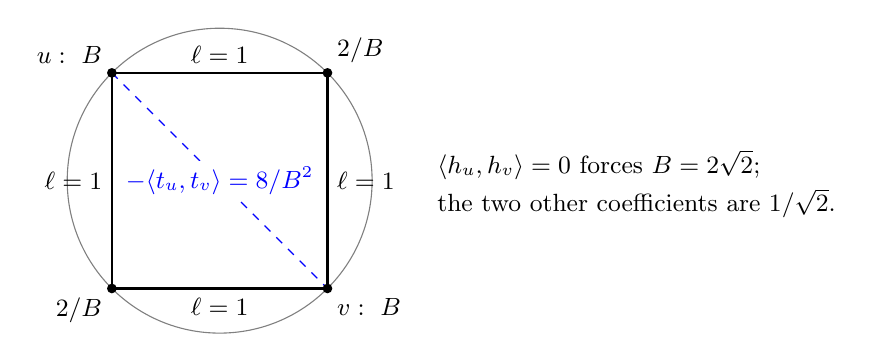
\begin{tikzpicture}[>=Latex,font=\small,scale=.88]
 \draw[gray] (0,0) circle(2.2);
 \coordinate (U) at (135:2.2); \coordinate (X) at (45:2.2);
 \coordinate (V) at (-45:2.2); \coordinate (Y) at (-135:2.2);
 \draw[thick] (U)--(X)--(V)--(Y)--cycle;
 \draw[dashed,blue] (U)--(V);
 \foreach \P in {U,X,V,Y}{\fill (\P) circle(2pt);}
 \node[above left] at(U) {$u:\ B$};
 \node[above right] at(X) {$2/B$};
 \node[below right] at(V) {$v:\ B$};
 \node[below left] at(Y) {$2/B$};
 \path (U)--node[above] {$\ell=1$}(X);
 \path (X)--node[right] {$\ell=1$}(V);
 \path (V)--node[below] {$\ell=1$}(Y);
 \path (Y)--node[left] {$\ell=1$}(U);
 \node[blue,fill=white,inner sep=2pt] at(0,0) {$-\ip{t_u}{t_v}=8/B^2$};
 \node[align=left,anchor=west] at(3,-.05)
 {$\ip{h_u}{h_v}=0$ forces $B=2\sqrt2$;\\[3pt]
  the two other coefficients are $1/\sqrt2$.};
\end{tikzpicture}
\caption{A decorated ideal quadrilateral, drawn in a schematic Klein
disc. Coefficients use the actual cusp-opposite normalization. Its
opposite-product identity will exclude the equality carrier.}
\label{fig:quad}
\end{figure}

\section{Exact defects and actual opposite-facet witnesses}\label{sec:witness}

We give the shared counting and geometric argument once, for a facet
$A^d$ of an ideal $P^{d+1}$ with $d=3$ or $4$. Let $m=\VV(A)$,
$N_i$ count outside vertices with $i$ neighbors in $A$, and $q$ count
edges of $A$ whose outgoing two-face is not a triangle.

\begin{lemma}[Exact outside partition]\label{lem:partition}
With the notation above,
\begin{equation}\label{eq:partition}
 N_1=2q,\qquad
 \VV(P)=(1+2^{d-2})m+N_0+q.
\end{equation}
\end{lemma}
\begin{proof}
Capacity gives $i\le2$ and $N_1+2N_2=2^{d-1}m$.
There are $2^{d-2}m$ edges of $A$. For an edge $uv$ the outgoing
two-face is triangular exactly when $\ip{h_u}{h_v}=-1$.
Indeed $h_u+h_v$ is then a feasible future null vector. The three
side halfplanes cut out the ideal triangle, and every other chamber
halfspace contains its three vertices and their convex hull.

Conversely an outside vertex with two $A$-neighbors puts those
neighbors at the two contact corners of one edge of its box, by the
proof of Lemma~\ref{lem:capacity}. Its $d-1$ common vertical walls
cut out the outgoing triangle, and $A$ cuts its remaining side.
The edge of $A$ determines this face and its third vertex uniquely.
Thus $N_2=2^{d-2}m-q$ is an equality, proving both formulas.
\end{proof}

Call a vertex of $A$ \emph{good} when all its $d-1$ opposite-pair
coefficients relative to $t_u=n+h_u$ are $<2$, and let $G$ count them.
\begin{lemma}[Good opposite facets]\label{lem:goodwitness}
A good $h_u$ is orthogonal to no other cusp-opposite facet $h_v$.
Every vertex of $h_u$ other than $u$ and its $2^{d-1}$ neighbors belongs
to $N_0$. At an $N_0$ vertex, at most two good $h_u$ occur. Consequently
\begin{equation}\label{eq:goodwitness}
 G\le2N_0\quad(d=3),\qquad 9G\le2N_0\quad(d=4).
\end{equation}
The witness conclusion remains true for a nongood $h_u$ if its
nonorthogonality to every other $h_v$ has been proved separately.
\end{lemma}
\begin{proof}
If $h_u\perp h_v$, then $\ip{t_u}{t_v}=-1$, so $u,v$ are not
adjacent by \eqref{eq:edgeproduct}. They share at most $d-2$ facets
of $A$. Otherwise among $d-1$ shared facets either an opposite pair
is asymptotic only at $u$, or all are mutually orthogonal and their
actual common one-face contains both $u,v$, making them adjacent.
At least one opposite pair through $u$ therefore misses $v$ entirely.
Its two products with $t_v$ are strictly negative and at most $-1$
by the actual-wall gap. Pairing its sum $\alpha t_u$ with $t_v$
forces $\alpha\ge2$, a contradiction.

Let $w\in h_u$ be a nonneighbor of $u$. It lies outside $A$ because
the two supporting hyperplanes meet only at $u$. If $w$ had an
$A$-neighbor $v$, the outgoing edge $wv$ would lie in $h_v$.
At $w$ the incident $h_u,h_v$ cannot be orthogonal; they must be
opposite walls in its rectangular box. With $w$ at infinity,
$A$'s hemisphere is tangent to those parallel walls at the known
actual points $u,v$ (Figure~\ref{fig:box}). Its radius is half their
separation and its tangency points have the same other coordinates.
Since $v$ is a box corner, $u$ is also one. The geodesic $uw$ is
feasible against every wall by convexity; $h_u$ and the other
$d-1$ common vertical walls define it as an actual edge. This
contradicts the choice of $w$.

For $d=3$, $h_u$ has at least six vertices and degree four at $u$,
leaving at least one witness. For $d=4$, Lemma~\ref{lem:capacity}
applied inside $h_u$ gives at least $3\cdot6=18$ vertices; its eight
neighbors at $u$ leave at least nine witnesses. Any three distinct
faces of a rectangular box include an orthogonal pair, so at most
two good $h_u$ can meet an $N_0$ vertex. Count these incidences.
Only the first paragraph used goodness; the stated extension follows.
\end{proof}

\section{A positive four-dimensional cusp defect}\label{sec:defect}

\begin{theorem}\label{thm:plus3}
If $R$ is a three-facet of an ideal right-angled four-polytope $Q$,
then $\VV(Q)\ge3\VV(R)+3$.
\end{theorem}
\begin{proof}
Put $m=\VV(R)$. At a cusp of $R$ the two pair coefficients
$\alpha,\beta$ each occur twice among its four polygon corners.
Every polygon has two small corners by Lemma~\ref{lem:polygon}.
At least $\max(0,8-2q)$ triangular faces have no exceptional edge,
since an edge lies in two polygons; these have three small corners.
Thus
\[
 S\ge2(m+2)+\max(0,8-2q),\qquad S\le2m+2G,
\]
and $G\ge2+\max(0,4-q)$. By Lemma~\ref{lem:goodwitness}, $2N_0\ge G$.
The exact defect is $\VV(Q)-3m=N_0+q$, so it is at least
\[
 q+\left\lceil\frac{2+\max(0,4-q)}2\right\rceil\ge3.
\]
For $q=0,1,2,3$ the lower bounds are $3,4,4,5$; for $q\ge4$
the lower bound is at least $q+1\ge5$.
\end{proof}

\section{The eleven-vertex equality cannot occur}\label{sec:equality}

\begin{lemma}[Six vertices force square cusps]\label{lem:octasquare}
An ideal right-angled three-polyhedron with six vertices has octahedral
graph and square cusp rectangles.
\end{lemma}
\begin{proof}
Its degree-four simple graph is the complete six-vertex graph minus a
perfect matching. Euler gives eight triangular faces. Send a vertex
$u$ to infinity and its nonneighbor $w$ to zero in upper half-space.
The vertical walls at $u$ bound
$[x_-,x_+]\times[y_-,y_+]$, with zero strictly inside, and its four
neighbors are the corners. The remaining facet across $x=x_+$
contains $w$ and that side's two corners. Right angles put the
hemisphere center on $x=x_+$; its other center coordinate is
$(y_-+y_+)/2$ and its radius $(y_+-y_-)/2$. Passing through zero
gives $x_+^2=-y_-y_+$. The opposite side gives the same equation
for $x_-^2$, so $x_-=-x_+$. The horizontal pair similarly gives
$y_-=-y_+$ and $y_+=x_+$. The rectangle is square. This is a direct
local proof, not a classification or rigidity assumption about $Q$.
\end{proof}

\begin{theorem}\label{thm:eleven}
If an ideal right-angled four-polytope has a three-facet with eleven
vertices, then it has at least thirty-seven vertices.
\end{theorem}
\begin{proof}
Suppose equality in Theorem~\ref{thm:plus3} gives $\VV(Q)=36$.
Its integer defect inequalities force
\[
 q=0,\qquad N_0=3,\qquad G=6.
\]
Every triangle of $R$ has coefficients one. If $T$ is their number,
the small-corner bounds now give
$2(11+2)+T\le S\le2\cdot11+2\cdot6=34$.
Equation~\eqref{eq:threeEuler} implies exactly eight triangles and
five quadrilaterals, with no larger face. Equality also makes every
nongood cusp have exactly one small coefficient and one coefficient
at least two.

Each of the six good opposite facets $h_u$ supplies at least one
$N_0$ witness by Lemma~\ref{lem:goodwitness}, and at most two occur
at any $N_0$ vertex. The total good incidence is exactly six.
All vertices of a good $h_u$ beyond $u$ and its four neighbors
are witnesses, so it has exactly six vertices. By
Lemma~\ref{lem:octasquare}, its cusp at $u$ is square. Its four
incident normals are precisely the same four normals used by $R$
at $u$, at the same fixed $t_u$ scale. Therefore
\begin{equation}\label{eq:goodEqual}
 \alpha_u=\beta_u\quad\hbox{at each good vertex of }R.
\end{equation}
No such six-vertex assertion has been made for a nongood facet.

We claim all eleven $h_u$ are pairwise nonorthogonal. The good case
is Lemma~\ref{lem:goodwitness}. Otherwise suppose $h_u\perp h_v$
with $u$ nongood, and write $A<2\le B$ for its coefficients.
Then $-\ip{t_u}{t_v}=1$, so $u,v$ are nonadjacent. The two facet
normals summing to $At_u$ cannot both miss $v$, or their products
with $t_v$ would force $A\ge2$. Thus $v$ is on one of those polygonal
facets through $u$. Its intrinsic corner coefficient at $u$ is the
OTHER coefficient $B$. It cannot be a triangle; it is a quadrilateral,
and $v$, nonadjacent to $u$, is its opposite vertex. Lemma~\ref{lem:quad}
forces $B=2\sqrt2$, with coefficient $1/\sqrt2$ at its other two
vertices.

At either of these two vertices, goodness gives both coefficients
$1/\sqrt2$ by \eqref{eq:goodEqual}; nongoodness makes the other
coefficient at least two. Neither coefficient is one. No triangle
can meet it, so each vertex belongs to four quadrilateral facets.
Only five quadrilateral facets exist. Their two four-element incident
sets therefore share at least three. But among any three facets at
a rectangular ideal cusp there is an opposite pair, whose hyperplanes
share only that cusp. Two distinct vertices cannot share those three
facets. This proves the claim.

Now apply the extended witness conclusion of
Lemma~\ref{lem:goodwitness} to ALL eleven $h_u$: each has a vertex
beyond $u$ and its four neighbors, which must lie in $N_0$ because
its $h_u$ is orthogonal to no other opposite facet. At an $N_0$ cusp
at most two pairwise nonorthogonal facets occur. Thus $11\le2N_0=6$,
the contradiction. See Figure~\ref{fig:equality}.
\end{proof}

\begin{figure}[tb]
\centering
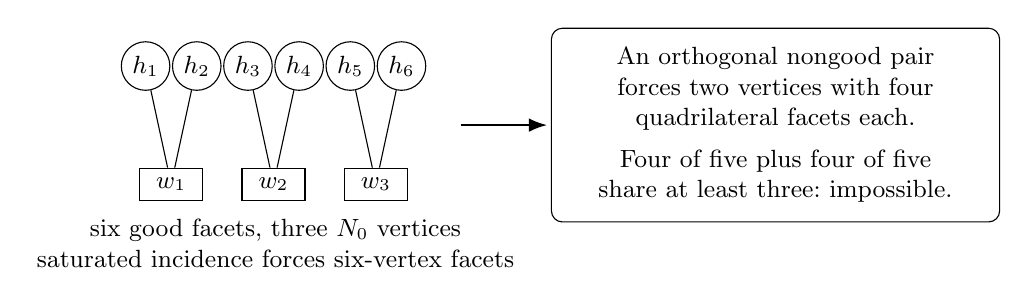
\begin{tikzpicture}[>=Latex,font=\small]
 \foreach \i in {1,...,6}{
  \node[draw,circle,inner sep=2pt] (g\i) at ({.65*(\i-1)},1.5) {$h_{\i}$};}
 \foreach \i in {1,...,3}{
  \node[draw,rectangle,minimum width=.8cm] (w\i) at ({1.3*(\i-1)+.325},0) {$w_{\i}$};}
 \draw (g1)--(w1) (g2)--(w1) (g3)--(w2) (g4)--(w2)
       (g5)--(w3) (g6)--(w3);
 \node[align=center] at(1.65,-.75)
   {six good facets, three $N_0$ vertices\\saturated incidence forces six-vertex facets};
 \draw[->,thick] (4, .75)--(5.1,.75);
 \node[draw,rounded corners,text width=5.2cm,align=center,inner sep=7pt]
  at(8,.75) {An orthogonal nongood pair forces two vertices
  with four quadrilateral facets each.\\[4pt]
  Four of five plus four of five share at least three:\ impossible.};
\end{tikzpicture}
\caption{The equality argument counts only the six good facets before
using their square cusps. The final witness count is extended to all
eleven facets only after pairwise nonorthogonality is established.}
\label{fig:equality}
\end{figure}

\section{Five-dimensional propagation}\label{sec:fiveprop}

\begin{theorem}\label{thm:fiveprop}
For every four-facet $Q$ of an ideal right-angled five-polytope $P$,
with $m=\VV(Q)$ and $f=\FF(Q)$,
\begin{equation}\label{eq:fiveprop}
 3\VV(P)\ge13m+6f.
\end{equation}
\end{theorem}
\begin{proof}
The exact outside partition is $\VV(P)=5m+N_0+q$.
The six intrinsic normals through a $Q$-cusp form three opposite
pairs. Each pair coefficient occurs four times among its twelve
polygon corners. Thus $S\le8m+4G$.

The degree-eight graph and Euler give $r=3m+f$ polygonal two-faces.
Their corner incidence is $12m$, so their total defect beyond
triangles is $12m-3r=3(m-f)$. Hence their triangle count satisfies
$T\ge r-3(m-f)=4f$. An exceptional edge belongs to exactly three
two-faces, so at least $\max(0,T-3q)$ triangles are unexceptional.
Lemma~\ref{lem:polygon} consequently gives
\[
 S\ge2r+\max(0,T-3q)\ge6m+6f-3q,
 \qquad 4G+3q\ge6f-2m.
\]
The $d=4$ case of Lemma~\ref{lem:goodwitness} gives $9G\le2N_0$.
In particular $4G\le8N_0/9\le3N_0$. Substitution into the last
inequality yields $3(N_0+q)\ge6f-2m$, proving
$3\VV(P)\ge15m+6f-2m$.
\end{proof}

\section{The carrier bridge and the dimension-five bounds}\label{sec:carrier}

For an ideal right-angled four-polytope define
\[
 \kappa(Q)=3\VV(Q)-4\FF(Q)+24.
\]
We distinguish one internal companion theorem from published inputs.

\begin{proposition}[Internal small-facet bridge]\label{prop:bridge}
An entirely ideal right-angled four-polytope all of whose three-facets
have at most ten vertices is an opposite-restricted chain of regular
ideal $24$-cells. A chain of $k$ cells has $\kappa=2-2k\le0$.
Thus $\kappa(Q)>0$ forces a three-facet with at least eleven vertices.
\end{proposition}

This is the internal companion result, not a published classification of
arbitrary four-polytopes. Its complete proof is in the unified ideal-four
manuscript~\cite{Internal4} and its named ten-vertex extension.
The external small-dimensional input is the complete ideal right-angled
three-polyhedron list through ten vertices: the octahedron, its
triangular-face double, the square and pentagonal antiprisms, and the
ten-vertex octahedrite in Kolpakov's Figure~7~\cite{K}, with the standard
three-dimensional realization uniqueness. The internal proof first
derives the antiprism and octahedrite cusp rectangles, excludes them
from this restricted facet spectrum by compatible box ratios and
same-ridge neighbor constraints, and then constructs the octahedral
sections and cuts proving the chain theorem. No unrestricted garland
assertion is used. We cite that already written structural proof rather
than duplicate it in a size-bound paper.

\begin{lemma}[Positive carrier]\label{lem:carrier}
Every ideal right-angled five-polytope has a four-facet $Q$ with
$\kappa(Q)>0$. Such a facet satisfies $\VV(Q)\ge37$ and $\FF(Q)\ge25$.
\end{lemma}
\begin{proof}
Write $(v,e,r,g,f)$ for the five-polytope's face counts. Its four-box
links give $e=8v$, total three-face vertex incidence $24v$, and total
four-facet vertex incidence $8v$. Every ideal right-angled three-face
has two more facets than vertices; every two-face has three three-
cofaces. Thus $3r=24v+2g$. Euler on the boundary four-sphere gives
$g=3v+3f-6$. Each three-face has two four-cofaces, and therefore
\begin{equation}\label{eq:kappasum}
 \sum_Q\kappa(Q)=3(8v)-4(2g)+24f=48.
\end{equation}
Choose a positive term and apply Proposition~\ref{prop:bridge}.
It contains a three-facet $R$ with $M\ge11$ vertices. If $M=11$,
Theorem~\ref{thm:eleven} gives $\VV(Q)\ge37$; if $M\ge12$,
Theorem~\ref{thm:plus3} already gives $\VV(Q)\ge39$.
Separately, Lemma~\ref{lem:injection} applied to $R$ gives
\begin{equation}\label{eq:carrierFacets}
 \FF(Q)\ge1+\FF(R)+\VV(R)=2M+3.
\end{equation}
\end{proof}
The separate facet count is not inferred from a vertex count.

\begin{theorem}\label{thm:fivebounds}
Every entirely ideal finite-volume right-angled five-polytope satisfies
\[
 \FF(P)\ge63,\qquad \VV(P)\ge211.
\]
Every entirely ideal right-angled six-polytope has at least $275$ facets.
\end{theorem}
\begin{proof}
At the positive carrier, Lemma~\ref{lem:injection} gives
$\FF(P)\ge1+25+37=63$.
Theorem~\ref{thm:fiveprop} gives $3\VV(P)\ge13\cdot37+6\cdot25=631$,
hence $\VV(P)\ge211$. Every five-facet of an ideal six-polytope
satisfies both inequalities; another facet injection gives
$\FF(P^6)\ge1+63+211=275$.
\end{proof}

\section{Good-edge transport in dimension six}\label{sec:transport}

We next prove a universal relation between the six-dimensional face
counts. No arithmetic hypothesis or facet spectrum enters this section.
At an ideal cusp choose future null vectors $v,z$ with $\ip{v}{z}=-1$
and orthonormal positive $e_1,\ldots,e_5$ perpendicular to them.
Centering its box gives the ten outward unit normals
\begin{equation}\label{eq:frame}
 n_i^\pm=\pm e_i+\frac{w_i}{2}v,\qquad w_i>0.
\end{equation}
A sign vector $\epsilon\in\{\pm1\}^5$ specifies an actual edge through
the cusp. Call it good if all five two-faces containing it are triangles,
and call the cusp cubic if all its $w_i$ agree.

Put $S=\sum_iw_i^2$. The third wall of the triangle obtained by dropping
the $i$th edge-support wall is forced to be
\begin{equation}\label{eq:thirdwall}
 c_i^\epsilon=\frac{S-2w_i^2}{4w_i}v+\frac2{w_i}z
       +\sum_{j\ne i}\epsilon_j\frac{w_j}{w_i}e_j.
\end{equation}
Indeed its products with both $n_i^+,n_i^-$ are $-1$, its products with
the other four supporting normals are zero, and its square is one.
These are actual ambient facet normals: right angles make the wall
cutting the polygon side orthogonal to its supporting walls.

At a good edge the five $c_i^\epsilon$ are mutually orthogonal and
\begin{equation}\label{eq:endpoint}
 n_i^{\epsilon_i}+c_i^\epsilon=\frac{v_\epsilon}{w_i},\qquad
 v_\epsilon=\frac S4v+2z+\sum_j\epsilon_jw_je_j.
\end{equation}
Direct products give $v_\epsilon^2=0$ and
$\ip{v}{v_\epsilon}=-2$. Its positive-sum expression makes it feasible
against every other actual wall; against its summands its product is
zero. It lies on the same supporting edge as $v$ and is its second
ideal endpoint. The ten distinct displayed normals fill its box link.
Their opposite sums in this normalization are $v_\epsilon/w_i$, so its
new widths are $1/w_i$. Good edges preserve cubicity in both directions.

\begin{lemma}\label{lem:goodedge}
At a noncubic cusp at most sixteen of its thirty-two edges are good.
If $g$ counts good edges and $t$ triangular two-faces at a cusp, then
$t\le64+g/2$, and therefore $t\le72$ at a noncubic cusp.
\end{lemma}
\begin{proof}
Suppose two good sign vectors differ only in direction $k$. For $i\ne k$
their two third walls have product $1-2w_k^2/w_i^2$. Both are
orthogonal to the common $c_k$ and the three unchanged supporting
normals. Product zero would give six mutually orthogonal actual walls
and a finite vertex. The gap of Lemma~\ref{lem:projection} forces
$1-2w_k^2/w_i^2\le-1$, so $w_k\ge w_i$ for every $i$.
At a noncubic cusp a nonmaximal direction pairs all thirty-two signs
and at most one member of each pair is good. Thus $g\le16$.
The five-cube has eighty edges. Every nongood cube vertex touches a
nontriangular link edge, so $2(80-t)\ge32-g$.
\end{proof}

At a cubic cusp normalize $w_i=1$. Then $v$ is canonical, the sum of
any opposite pair of actual unit normals. The vector
\[
 h=z-v/8,\qquad h^2=1/4,\qquad \ip{h}{v}=-1
\]
is independent of signed permutations of the centered frame. Across a
good edge define $e_i'=n_i^{\epsilon_i}-v_\epsilon/2$ and
$z'=h+v_\epsilon/8$. Their products give a new centered orthonormal
frame, $z'^2=0$, $\ip{z'}{v_\epsilon}=-1$, and
$h=z'-v_\epsilon/8$. Thus $h$ is constant on each finite component
of cubic cusps connected by good edges, including around cycles.

Choose a future null $Z\perp h$ in each component. Set
$E(v)=-\ip{Z}{v}>0$ and $p_i=\ip{Z}{e_i}/E(v)$.
The energy is nonzero because $Z\perp h$ but $\ip{v}{h}=-1$.
The equations $Z^2=\ip{Z}{h}=0$ give
\begin{equation}\label{eq:ratio}
 \sum_i p_i^2=\frac14,\qquad
 \frac{E(v_\epsilon)}{E(v)}=\frac32-\sum_i\epsilon_i p_i.
\end{equation}
Every formal ratio is positive even when that sign vector is not an
actual good edge: its formal endpoint is future null and has $h$-product
$-1$, so it is not parallel to $Z$.

\begin{figure}[tb]
\centering
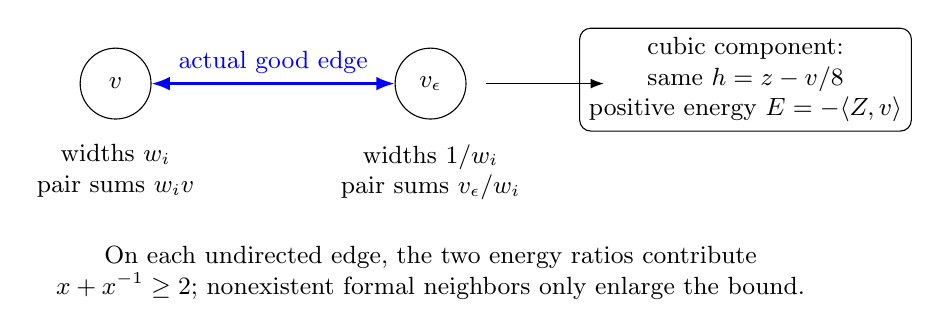
\begin{tikzpicture}[>=Latex,font=\small]
 \node[draw,circle,minimum size=9mm] (v) at(0,0) {$v$};
 \node[draw,circle,minimum size=9mm] (u) at(4,0) {$v_\epsilon$};
 \draw[<->,thick,blue] (v)--node[above] {actual good edge}(u);
 \node[below,align=center] at(0,-.65) {widths $w_i$\\pair sums $w_iv$};
 \node[below,align=center] at(4,-.65) {widths $1/w_i$\\pair sums $v_\epsilon/w_i$};
 \node[draw,rounded corners,align=center] at(8,.05)
  {cubic component:\\same $h=z-v/8$\\positive energy $E=-\ip{Z}{v}$};
 \draw[->] (4.7,0)--(6.2,0);
 \node[align=center] at(4,-2.4)
  {On each undirected edge, the two energy ratios contribute\\
   $x+x^{-1}\ge2$; nonexistent formal neighbors only enlarge the bound.};
\end{tikzpicture}
\caption{Actual endpoint transport and the unweighted reciprocal-pair
sum. Width transport is exact; the thirty-two formal directions are
used only as an upper relaxation after every ratio is positive.}
\label{fig:transport}
\end{figure}

\section{Sharp reciprocal averaging and six-dimensional vertices}\label{sec:reciprocal}

\begin{lemma}\label{lem:reciprocal}
For independent uniform signs and $\sum_{i=1}^5p_i^2=1/4$,
\begin{equation}\label{eq:reciprocal}
 \mathbb E\frac1{3/2-\sum_i\epsilon_i p_i}\le\frac{103}{132}.
\end{equation}
Equality holds exactly when all $p_i^2=1/20$.
\end{lemma}
\begin{proof}
Put $a_i=p_i^2$, $X=\sum_i\sqrt{a_i}\epsilon_i$, $\mu=3/2$.
On the compact simplex $a_i\ge0$, $\sum_i a_i=1/4$, one has
$|X|\le\sqrt5/2<\mu$. Sign symmetry and a uniformly convergent
positive series give
\[
 \mathbb E(\mu-X)^{-1}
 =\mu^{-1}\sum_{k\ge0}\mu^{-2k}\mathbb E X^{2k}.
\]
Fix two squares $a,b$, their sum $s$, and the remaining independent
symmetric sum $R$. For $Y=\sqrt a\epsilon+\sqrt b\eta$,
\[
 \mathbb E Y^{2j}=\sum_{\ell=0}^{\lfloor j/2\rfloor}
 \binom j{2\ell}s^{j-2\ell}(4ab)^\ell.
\]
Balancing $a,b$ increases every even moment. Expanding
$\mathbb E(R+Y)^{2k}$ has only nonnegative even terms, so it too
increases. The fourth moment increases strictly by $(a-b)^2$ if
$a\ne b$. The reciprocal average is continuous and has a compact
maximizer, including on the boundary; no maximizer can have unequal
squares. At equality, $X^2=5/4,9/20,1/20$ with multiplicities $2,10,20$.
Pairing opposite signs gives exactly
\[
 \frac32\left(\frac{1/16}{1}+\frac{5/16}{9/5}
                         +\frac{5/8}{11/5}\right)=\frac{103}{132}.
\]
This proves the global inequality and its equality characterization,
not merely a sampled finite-direction maximum.
\end{proof}

At a cubic vertex the positive function $1/E$ has outgoing ratio sum
at most $32\cdot103/132=824/33$, allowing all formal neighbors.
Summing over each good-edge component, every actual undirected edge
contributes a reciprocal pair at least two. The unweighted total good
degree of cubic cusps is therefore at most $(824/33)V_c$.
Lemma~\ref{lem:goodedge} then bounds their triangular corners by
$(64+412/33)V_c=(2524/33)V_c$; the noncubic bound $72$ is smaller.
If $T$ is the number of triangular two-faces of $P^6$, each has three
cusps, so
\begin{equation}\label{eq:trianglebound}
 3T\le\frac{2524}{33}V,\qquad V=\VV(P^6).
\end{equation}

\begin{theorem}\label{thm:sixbounds}
Every entirely ideal finite-volume right-angled six-polytope with $F$
facets and $V$ vertices satisfies
\[
 F\ge275,\qquad V\ge\left\lceil\frac{6039F}{272}\right\rceil
 \ge6106.
\]
\end{theorem}
\begin{proof}
Write $a_j=f_j(P)$, $a_0=V$, $a_5=F$. Its box links give $a_1=16V$.
Summing the five-dimensional identity $g=3v+3f-6$ over facets gives
$3a_3=30V+6a_4-6F$; Euler gives $a_2=25V+a_4-F$.
Polygon-cusp incidence is $80V$. Since nontriangles have at least
four corners,
\[
 T\ge4a_2-80V=20V+4(a_4-F).
\]
Together with \eqref{eq:trianglebound}, multiplying this lower bound
by THREE gives $a_4-F\le136V/99$. Each five-facet has at least
sixty-three four-facets by Theorem~\ref{thm:fivebounds}; every four-face
has two five-cofaces. Thus
\[
 \frac{61}{2}F\le a_4-F\le\frac{136}{99}V,
 \qquad 272V\ge6039F.
\]
The facet bound $F\ge275$ was already proved. Finally
$6039\cdot275=1660725$, whereas
$272\cdot6105=1660560<1660725\le1660832=272\cdot6106$.
\end{proof}

The reciprocal constant is sharp for formal cusp-frame averages. No
attainment by an actual polytope, or optimality of the size bounds, is
claimed.

\section{A restriction on mixed-dimensional boundaries}\label{sec:mixed}

Here the additional premises are published. The strict
Nikulin--Khovanskii inequality for polytopes simple at edges is
\[
 \frac1{f_k(P)}\sum_{E\in\Omega_k(P)}f_l(E)
 <\binom{n-l}{n-k}
 \frac{\binom{\lfloor n/2\rfloor}{l}+\binom{\lceil n/2\rceil}{l}}
 {\binom{\lfloor n/2\rfloor}{k}+\binom{\lceil n/2\rceil}{k}},
 \quad 0\le l<k\le\lceil n/2\rceil.
\]
The right-angled hypotheses and this precise range are recorded in
Alexandrov~\cite[\S\S2,6]{A} and Egorov~\cite{E}. For $n=11,12$,
the permitted choices $(k,l)=(5,4),(6,5)$ give strict averages twenty
and forty-two. Faces of dimension at least three remain finite-volume
and right-angled, so both applications are valid even with mixed vertices.

The general five-dimensional facet minimum sixteen is Dufour's
$f_4\ge1+\nu_4$ with $\nu_4=15$, stated in~\cite[Lemma~2.3]{E}.
The six-dimensional minimum twenty-seven is Dufour's
$f_5\ge1+\nu_5$ with $\nu_5\ge26$, stated in~\cite[Proposition~6.5]{A}.
Their noncompact scope covers these dimensions because compact
right-angled polytopes have dimension at most four, by the published
Potyagailo--Vinberg theorem. The original subscription Dufour proof was
not independently available here; we use these precisely stated premises,
not an asserted new proof of that theorem.

Let $N_k$ count all $k$-faces and $I_k$ the entirely ideal ones. Our
new necessary counts give
\[
 16N_5+47I_5\le\sum_{E\in\Omega_5(P)}f_4(E)<20N_5,
 \qquad \frac{I_5}{N_5}<\frac4{47},
\]
and
\[
 27N_6+248I_6\le\sum_{E\in\Omega_6(P)}f_5(E)<42N_6,
 \qquad \frac{I_6}{N_6}<\frac{15}{248}.
\]
They are coupled necessary incidence restrictions, not contradictions.
In particular the right-angled dimension ceilings remain six for the
entirely ideal class and twelve for the general finite-volume class.

\section{Proof interfaces and verification scope}\label{sec:verification}

The small-facet bridge of Proposition~\ref{prop:bridge} is an internal
companion theorem with explicit published three-dimensional inputs;
it is not an external axiom or a classification of arbitrary ideal
four-polytopes. The outside capacity, fixed-scale spinor proof,
positive defect, eleven-vertex equality exclusion, propagation, actual
good-edge transport, and all-moment reciprocal proof are human proofs
given in this paper. Their separate internal mathematical reviews are
indexed in the preparation map accompanying this source.

Existing exact scripts check frame identities, grouped sign sums and
older rational consequences. Such finite checks do not replace the
universal proofs for every width or polygon. Existing conditional Lean
modules cover earlier arithmetic interfaces with their geometric
premises explicit. No full formal proof of the new geometric chain or
of the $63/211$ and $275/6106$ constants is claimed by this revision.
Source reviews, exact execution records and typesetting records are kept
separately; successful typesetting is not a mathematical proof.
See \path{docs/ideal_right_angled_six_face_constraints_preparation_20261019.md}
for the source archive, theorem map, frozen dependencies and execution scope.

\begin{thebibliography}{9}
\bibitem{K} A. Kolpakov, \emph{On the optimality of the ideal right-angled
24-cell}, Algebraic \& Geometric Topology 12 (2012), 1941--1960.
\url{https://doi.org/10.2140/agt.2012.12.1941}.
\bibitem{A} S. Alexandrov, \emph{On ideal vertices of right-angled
hyperbolic polyhedra}, 2023. \url{https://arxiv.org/abs/2303.09533}.
\bibitem{E} A. Egorov, \emph{On lower bounds for the number of ideal
and finite vertices of right-angled hyperbolic polyhedra in dimensions
from 5 to 12}, 2026. \url{https://arxiv.org/abs/2603.29925}.
\bibitem{Internal4} Coxeter Polytopes Frontier Project,
\emph{Volume and structure of ideal right-angled four-polytopes},
internal companion manuscript, \path{manuscripts/ideal_ra4_volume_and_structure.tex},
with the separately reviewed extension
\path{results/ideal_ra4_ten_vertex_facet_exclusion_research_20261019.md}.
The three-dimensional small-facet classification is the stated external
input; the four-dimensional structural conclusions are internal proofs.
\end{thebibliography}
\end{document}
